\paragraph{State Machines}
\begin{itemize}
\item A state machine consists of
  \begin{itemize}
  \item State variables (encoding its state)
  \end{itemize}

\item Instructions
  \begin{itemize}
  \item transforming its state
  \end{itemize}
\end{itemize}


\paragraph{State-Machine Replication (or Active Replication)}
\begin{itemize}
\item Assumption
  \begin{itemize}
  \item Instructions of interpreter are deterministic!
  \item If replicas of interpreter get same inputs, they will go
    to the same state and produce the same output
  \end{itemize}
\end{itemize}

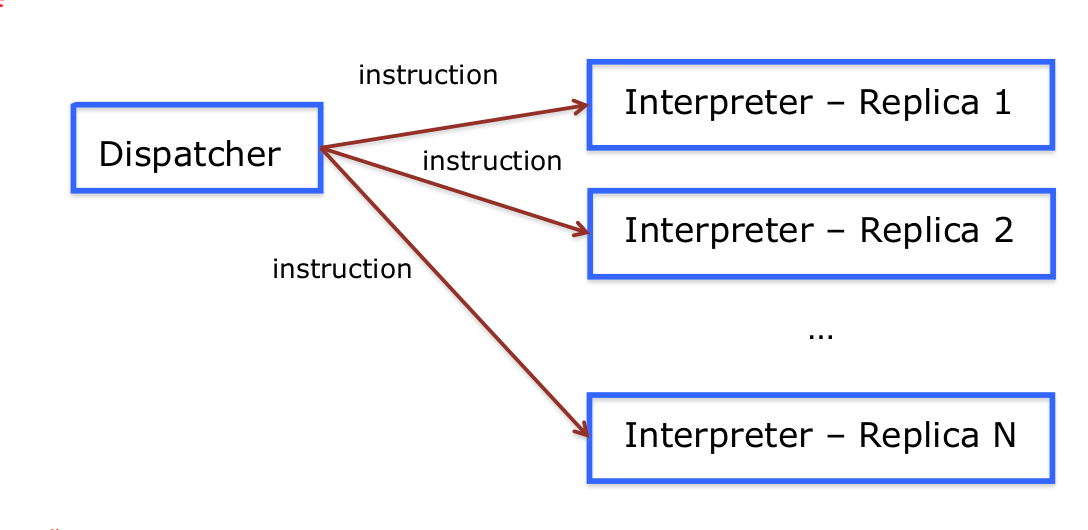
\includegraphics[scale=0.15]{graphics/dispatcher.png}


\paragraph{Multicast: Distributing the Dispatcher}
\begin{itemize}
\item Replicas implement \textbf{multicast} operation
  → internalize dispatcher
\item Must ensure \textbf{atomic} operation execution on all
  replicas
  \begin{itemize}
  \item \textbf{All-or-nothing:} either in all correct replicas or
    none
    \begin{itemize}
    \item also called \textbf{Agreement}
    \end{itemize}

  \item \textbf{Before-or-after:} Equivalent to a total order
    \begin{itemize}
    \item also called \textbf{Order}
    \end{itemize}

  \item With at most $f$ failures:
    \begin{itemize}
    \item  \textbf{Fail-stop:} requires at least N = $f$ + 1 replicas
    \item \textbf{Byzantine:} requires at least N = 2$f$ + 1 replicas
    \end{itemize}
  \end{itemize}
\end{itemize}

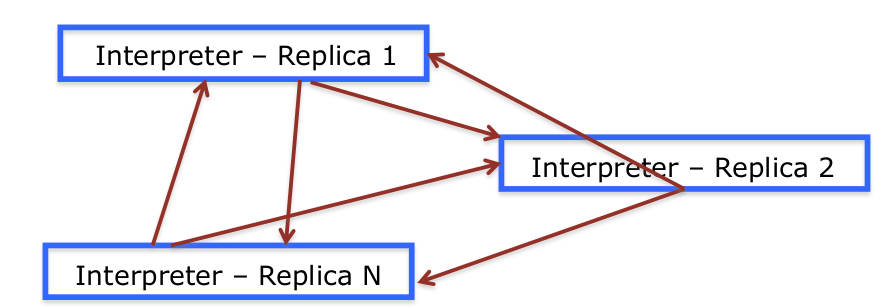
\includegraphics[scale=0.15]{graphics/multicast.png}

\paragraph{Totally Ordered Multicast (ISIS)}

\begin{minipage}{0.37\textwidth}
\begin{itemize}
\item Assume for now no failures
\item \textbf{Idea}
  \begin{itemize}
  \item Process 1 sends message with identified $i$ to group
  \item Every process $p$ replies with proposed \\
    $seq\# = \max(accepted_p, proposed_p) +1$
  \item Process 1 selects maximum number and sends it to group \\
    (Note: ties in numbering broken by process numbers)
  \end{itemize}
\end{itemize}
\end{minipage}%
\begin{minipage}{0.2\textwidth}
  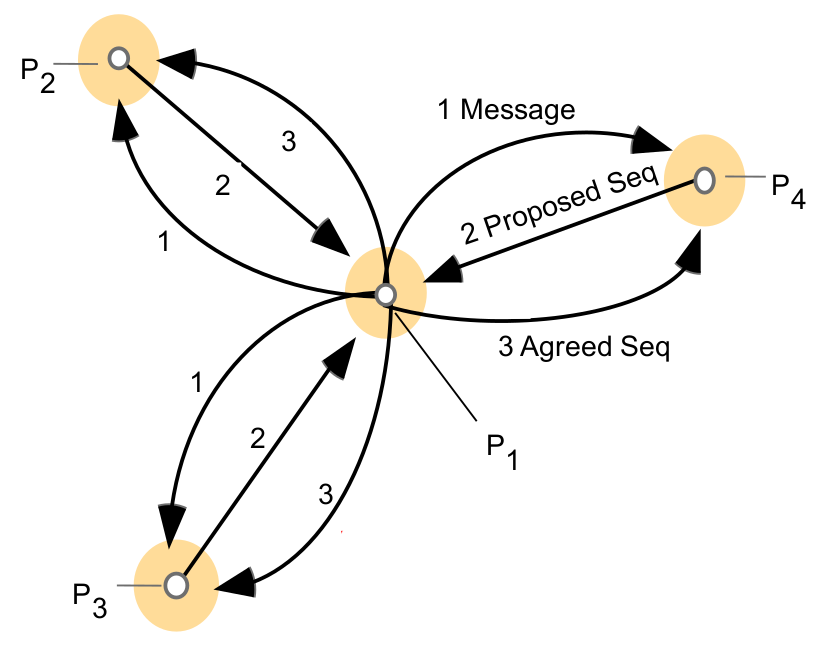
\includegraphics[scale=0.1]{graphics/isis.png}
\end{minipage}

\paragraph{Reliable and Totally Ordered Multicast?}
\begin{itemize}
\item if network is \textbf{asynchronous} and assuming \textbf{crash}
  failures, \textbf{guaranteeing} reliable \textbf{and} totally
  ordered multicast is \textbf{IMPOSSIBLE}

\item Fischer, Lynch, Patterson (FLP) result →
  Impossibility of Consensus
  \begin{itemize}
  \item Set of processes with single binary variable
  \item Want to decide outcome as 0 or 1 by just exchanging messages
  \item \textbf{Intuition:} cannot make the difference between
    crashed process and process running very slowly
  \item Adversary \textbf{delay} consensus indefinitely
  \item Does not mean that consensus cannot be reached in some cases!
  \end{itemize}
\end{itemize}

\begin{itemize}
\item \textbf{Solution 1:} Make model \textbf{fail-stop}, not crash
  \begin{itemize}
  \item Instead of asynchronous system, make system
    behave as a (partially) synchronous one with reliable
    failure detector, e.g., timeout
  \item Use failure detector to flag failed processes, no doubts
  \end{itemize}

\item \textbf{Solution 2:} Design
  \textbf{protocol that guarantees safety}, even if it cannot
  guarantee progress
  \begin{itemize}
  \item Paxos example of such a protocol
  \end{itemize}
\end{itemize}


\paragraph{Byzantine Generals}
\begin{itemize}
\item \textbf{Termination:} Eventually each process sets its
  decision variable
\item \textbf{Agreement:} The decision value of all the
   all correct processes is the same:
  if $p_i$ and $p_j$ are correct and have entered
  their decided state, then $d_i = d_j$ (for all $i,j = 1,...,N)$
\item \textbf{Integrity:} If the commander is correct, then all
  correct processes decide on the value that the commander proposed
\end{itemize}

\paragraph{Impossibility with Three Processes}
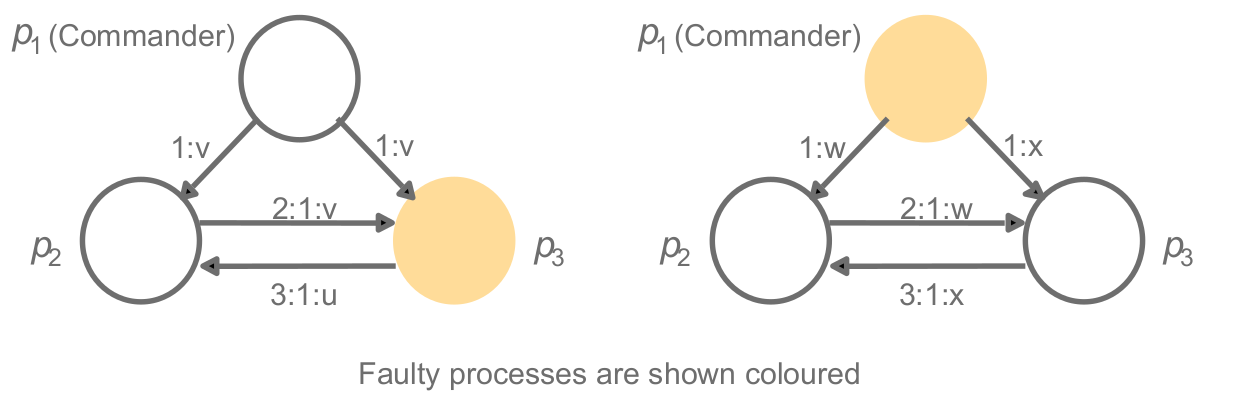
\includegraphics[scale=0.15]{graphics/byzantine-impossible.png}


\paragraph{Solution in Synchronous system}
\begin{itemize}
\item use two phases
  \begin{itemize}
  \item in phase 1 commander sends message
  \item in second round each process sends received message to others
    and then do majority vote
  \end{itemize}
\item If no majority (e.g. commander is compromised)
  , play it safe and do nothing
\end{itemize}


\paragraph{Distributed Transactions}
\begin{itemize}
\item Users should be able to write Xacts accessing multiple
  sites just like local Xacts

\item enforcing \textbf{ACID} class for distributed locking,
  recovery, and commit protocols

\item Hard to scale in number of sites in general
  \begin{itemize}
  \item Use partitioning / replication
    techniques for trade-offs
  \end{itemize}
\end{itemize}


\paragraph{Distributed Locking}
\begin{itemize}
\item How do we manage locks for objects across many sites?
\item \textbf{Centralized:} One site does all locking
  \begin{itemize}
  \item Vulnerable to single site failure
  \end{itemize}

\item \textbf{Distributed:} Locking for an object done at site
  where the object is stored
\end{itemize}

\paragraph{Distributed Deadlock Detection}
\begin{itemize}
\item Each site maintains a local waits-for graph
\item A global deadlock might exist even if the local
  graphs contain no cycles:

  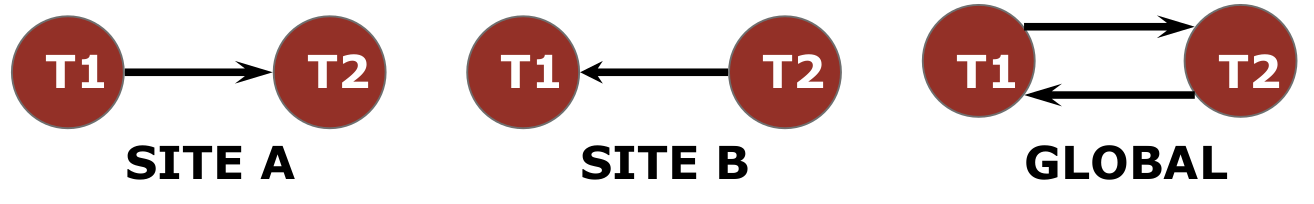
\includegraphics[scale=0.15]{graphics/global-deadlock.png}

\item Three solutions:
  \begin{itemize}
  \item \textbf{Centralized:} send all local graphs to one site
  \item \textbf{Hierarchical:} organize sites into a hierarchy and
    send local graphs to parent in the hierarchy
  \item \textbf{Timeout:} abort Xact if it waits too long
  \end{itemize}
\end{itemize}


\paragraph{Distributed Recovery}
\begin{itemize}
\item New issues:
  \begin{itemize}
  \item New kinds of failure, e.g. links and remote sites
  \item If ``sub-transactions'' of a Xact execute at different
    sites, all or none must commit
    → need a \textbf{commit protocol} to achieve this
  \end{itemize}

\item A log is maintained at each site, as in a centralized DBMS,
  and \textbf{commit protocol actions are additionally logged}
\end{itemize}


\paragraph{Two-Phase Commit (2PC)}

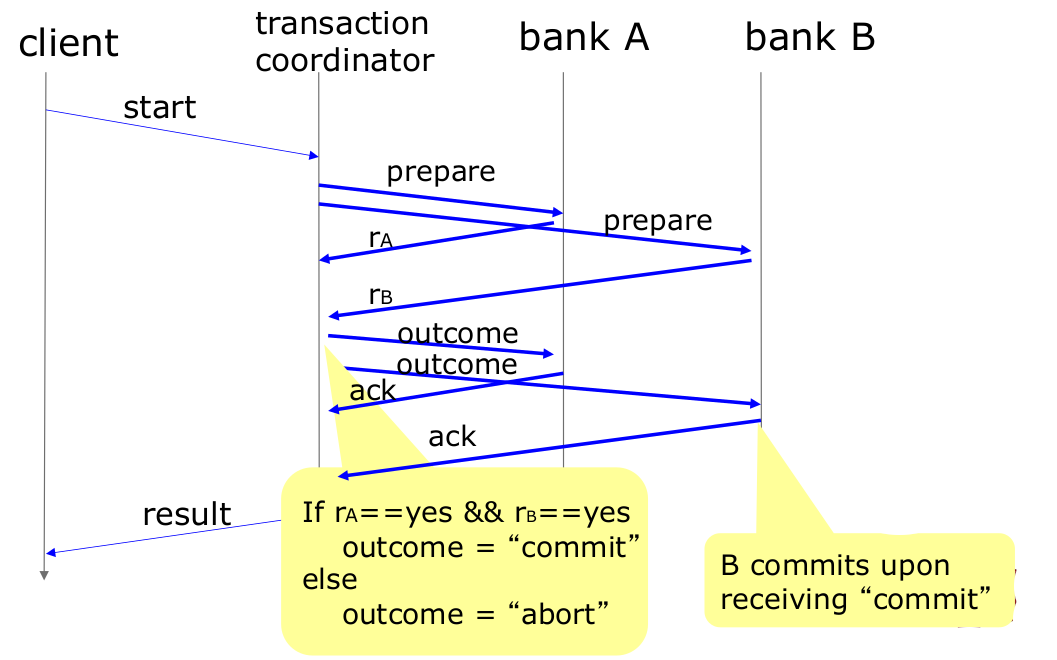
\includegraphics[scale=0.15]{graphics/two-phase-commit.png}

\paragraph{Comments on 2PC}
\begin{itemize}
\item Two rounds of communication: first \textbf{voting},
  then \textbf{termination}
  \begin{itemize}
  \item Both initiated by coordinator
  \end{itemize}

\item \textbf{Any site} can decide to \textbf{abort} an Xact

\item Every msg reflects a \textbf{decision} by the sender
  \begin{itemize}
  \item To ensure that this decision survives failures, it is first
    \textbf{recorded in the local log}
  \end{itemize}

\item All commit protocol log recs for an Xact contain Xactid and
  Coordinatorid
  \begin{itemize}
  \item The coordinator's abort/commit record also includes
    ids of all subordinates/cohorts
  \end{itemize}
\end{itemize}

\paragraph{Discussion of Failure Scenarios}
\begin{itemize}
\item Coordinator times out waiting for subordinate's ``yes/no''
  response
  \begin{itemize}
  \item coordinator can \textbf{not} unilaterally decide to commit
  \item coordinator \textbf{can} unilaterally decide to abort
  \end{itemize}

\item If subordinate $i$ responded with ``no'' ...
  \begin{itemize}
  \item it \textbf{can} unilaterally abort
  \end{itemize}

\item If subordinate $i$ responded with ``yes'' ...
  \begin{itemize}
  \item it can \textbf{not} unilaterally abort
    (since the coordinator might decide to commit)
  \item it can \textbf{not} unilaterally commit
  \end{itemize}
\end{itemize}


\paragraph{Restart After a Failure at a Site}
\begin{itemize}
\item If we have a commit or abort log rec for Xact T, but
  not an end rec, must redo/undo T
  \begin{itemize}
  \item If this site is the coordinator for T, keep sending
    \textbf{commit/abort} msgs to subs until \textbf{acks} received
  \end{itemize}

\item If we have a prepare log rec for Xact T, but not
  commit/abort, this site is a subordinate for T
  \begin{itemize}
  \item Repeatedly contact the coordinator to find status of T,
    then write \textbf{commit/abort} log rec; redo/undo T; and
    write \textbf{end} log rec
  \end{itemize}

\item If we don't have even a prepare log rec for T, unilaterally abort
  and undo T
  \begin{itemize}
  \item This site may be coordinator! If so, subs may send msgs
  \end{itemize}
\end{itemize}


\paragraph{Blocking}
\begin{itemize}
\item If coordinator for Xact T fails, subordinates who have
  voted yes cannot decide whether to commit or abort T until
  coordinator recovers
\item T is \textbf{blocked}
\item (one of the major problems of two-phase-commit)
\end{itemize}


\paragraph{Link and Remote Site Failures}
\begin{itemize}
\item If a remote site does not respond during the commit protocol
  for Xact T, either because the site failed or the link failed
\item If the current site is a subordinate, and has not
  yet voted yes, it should abort T
\item If the current site is a subordinate and has voted yes,
  it is blocked until the coordinator responds
\end{itemize}

\paragraph{2PC with Presumed Abort}
\begin{itemize}
\item When coordinator aborts T, it undoes T and removes it from
  the Xact table immediately
  \begin{itemize}
  \item Doesn't wait for \textbf{acks}; ``presumes abort'' if
    Xact not in Xact Table. Names of subs not recorded in \textbf{abort}
    log rec
  \end{itemize}

\item Subordinates do not send acks on abort
\item If subxact does not do updates, it responds to
  prepare msg with reader instead of yes/no
\item Coordinator subsequently ignores readers
\item If all subxacts are readers, 2nd phase not needed
\end{itemize}

% LocalWords:  Multicast multicast FLP Paxos Xacts Xact msg recs msgs
% LocalWords:  Xactid Coordinatorid acks subxact subxacts nd
